\begin{frame}{A Taxonomy of Repeated Games Models}
    \begin{figure}
        \tikzstyle{mybox} = [draw=gray!20, fill=white, very thick,
        rectangle, rounded corners, inner sep=10pt, inner ysep=10pt]
        \tikzstyle{fancytitle} = [fill=gray, text=white, rounded corners]
        \scalebox{0.7}{
        \begin{tikzpicture}
            \node [mybox] at (0, 0) (gen-mod){%
                \begin{minipage}{0.50\textwidth}
                    \vspace{-0.25cm}
                    \[ \Gamma^r = (N, \Theta, (D_i, S_i, u_i)_{i\in N}, q, p) \]
                \end{minipage}
            };
            \node [inner sep=0pt] (gen-mod-img) at (-4.4, 0.5){%
                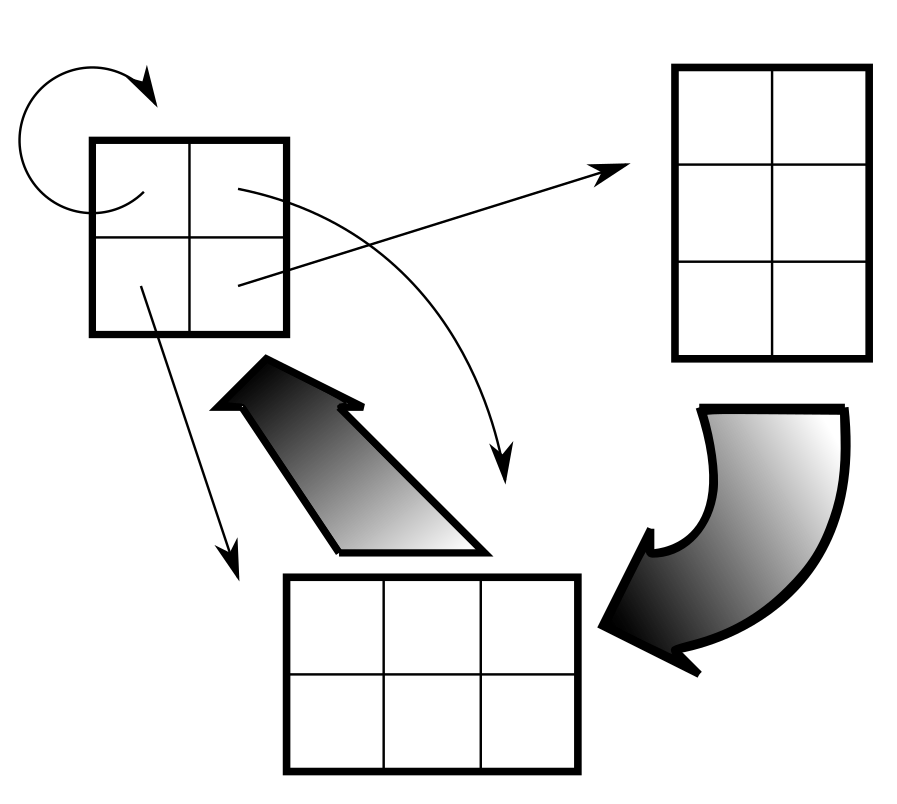
\includegraphics[width=0.25\textwidth]{img/stochastic.png}
            };
            
            \node [mybox] at (-4.5, -3) (mdp){%
                \begin{minipage}{0.40\textwidth}
                    {\color{green}Single-agent stochastic game}
                    \vspace{-0.25cm}
                    \[ |N| = 1. \]
                \end{minipage}
            };
            
            \node [mybox, draw=black] at (0, -7.5) (state){%
                \begin{minipage}{\textwidth}
                    {\color{green}At every round, every player knows the
                    current state of nature $\theta \in \Theta$.} \\
                    Informally, for each player $i \in N$, there exists some
                    state $w(s_i) \in \Theta$ such that the signal $s_i$ can
                    never occur unless the current state is $w(s_i)$.
                \end{minipage}
            };
            
            \node [mybox] at (4.5, -3.5) (std){%
                \begin{minipage}{0.60\textwidth}
                    \begin{itemize}
                        \item {\color{green}Only one possible state of
                        nature}
                        \[ |\Theta| = 1. \]
                        \item {\color{green}Players know all of each other's past
                        moves}
                        \[ S_i = \bigtimes_{j\in N-i} D_j. \]
                    \end{itemize}
                \end{minipage}
            };
            \node [inner sep=0pt] (gen-mod-img) at (7, -5.5){%
                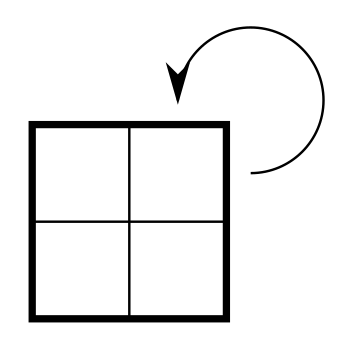
\includegraphics[width=0.20\textwidth]{img/std.png}
            };

            \node[fancytitle] at (gen-mod.north) {Stochastic Games (General Model)};
            \node[fancytitle] at (mdp.north) (mdp-title) {Markov Decision Processes};
            \node[fancytitle, fill=black] at (state.north) (state-title) {Complete State Information};
            \node[fancytitle] at (std.north) (std-title) {Standard Repeated Games};

            \draw[thick, -Latex] (gen-mod.west) -- (mdp-title.north);
            \draw[thick, -Latex] (gen-mod.south) -- (state-title.north);
            \draw[thick, -Latex] (gen-mod.east) -- (std-title.north);
        \end{tikzpicture}}
        \caption{A taxonomy of repeated game models.}
    \end{figure}
\end{frame}

\begin{frame}{Game with complete state information: definition}
    \metroset{block=fill}
    \begin{block}{Definition}
        A repeated game $\Gamma^r = (N,\Theta, (D_i,S_i,u_i)_{i\in N},q,p)$ has
        \textbf{complete state information} if, at every round, every player knows
        the current state of nature. That is, there is a function
        $\omega_i:S_i \rightarrow \Theta$ known by each player such that
        \begin{equation*}
            p(s,\hat{\theta} | d,\theta) = 0 \text{ if } \hat{\theta} \neq \omega_i(s_i)
        \end{equation*}
        $\forall s \in S, \forall \theta, \hat{\theta} \in \Theta, \forall d \in D$.
        So the signal $s_i$ can never occur unless the current state is $\omega(s_i)$.
    \end{block}

    \pause
    \textbf{{\color{green}Is the example of the Prisoner's Dilemma with the dice roll a game
    with complete state information?}} \\
    \pause
    Yes, each player knows whether the game is \textit{active} or \textit{stopped}.
\end{frame}

\begin{frame}{Stationary strategies}
    \metroset{block=fill}
    \begin{block}{Definition}
        In a repeated game, a game is said to be \textbf{stationary} iff the move probability
        depends only on the current state. That is there is a function $\tau_i : \Theta
        \rightarrow \Delta(D_i)$ such that:
        \begin{equation*}
	        \sigma_i^{[k]}(\cdot | s) = \tau_i(\cdot | \omega_i(s_i^{[k]}))
        \end{equation*}
        $\forall k, \forall s \in (S)^{\times k}$.
    \end{block}

    \pause
    \textbf{{\color{green}Is the Grim strategy proposed earlier stationary?}} \\
    \pause
    The Grim strategy \textbf{depends on past move} and not on the actual state. It
    is not stationary.
    \pause
    However, \textit{we can make this strategy stationary by using an equivalent model with larger
    state space}
    \begin{itemize}
        \item \textbf{Ac} : Active plays continuing (nobody has chosen \textit{defect} in the past).
        \item \textbf{Ad} : Active plays continuing (someone has chosen \textit{defect} in the past).
    \end{itemize}
\end{frame}

\note{
	Explain that this definition is only for game with complete state information
	
	Il faut connaître l'état pour etre stationnaire, si on ne connait pas l'état on
    ne pourra pas être stationnaire.

    At this point, update the first model of the RPD that was on the blackboard with this new
    augmented one.
}

\begin{comment}
\begin{frame}{Small example to understand complete state information}
    \textit{Consider the prisoner's dilemma game in a setting where player make decision
    based only on the last move of they adversary.}
    
    \note{This is contrary to decision theory to make this assumption. Some strategies can
    still be analyzed in that setting. (tit-for-tat)}

    \pause
    $\Rightarrow$ 4 different states : $\Theta = \{([C,c]), ([C,d]), ([D,c]), ([D,d])\}$

    \pause
    If both player play the \textbf{tit-for-tat} strategy. {\color{green} We can represent } the game like that:

    \begin{minipage}{0.7\linewidth}
    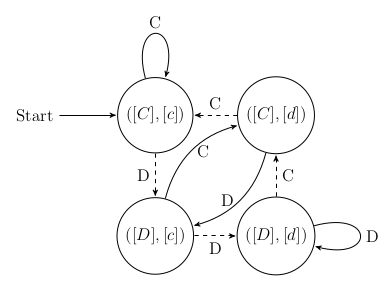
\includegraphics[width=0.9\linewidth]{img/titfortat.png}
    \end{minipage}
    \begin{minipage}{0.29\linewidth}
        \begin{itemize}
            \item Plain arrow if player 1 play tit-for-tat.
            \item Dashed arrow if player 1 play the opposite.
            \item Player 2 play tit-for-tat
        \end{itemize}
    \end{minipage}
\end{frame}
\end{comment}

\begin{frame}{Stationary Equilibria (1)}
    \begin{itemize}
        \item $\nu_i(\tau, \theta)$ is the expected $\delta$-discounted average for player $i$
        \begin{itemize}
            \item if players plan to use the stationary strategy profile $\tau$, and 
            \item the initial state of nature is $\theta$.
        \end{itemize}
        \item $Y_i(\tau, d_i, v_i, \theta, \delta)$ is the expected $\delta$-discounted average for
        player $i$
        \begin{itemize}
            \item if every players plan to implement $\tau$ excepts player $i$ that plays $d_i$, and
            \item the initial state of nature is $\theta$.
        \end{itemize}
    \end{itemize}

    \begin{small}
        \begin{eqnarray}
            Y_i(\tau, d_i, \nu_i, \theta, \delta) &=&
            \sum_{d_i \in D_i} \left( \prod_{j \in N-i} \tau_j(d_j|\theta) \right) \nonumber \\
            && \cdot  \left(  (1-\delta) u_i(d,\theta) + \delta \sum_{\hat{\theta} \in \Theta}
            \sum_{s \in S} p(s,\hat{\theta} |d,\theta) \nu_i (\hat{\theta}) \right)
        \end{eqnarray}  
    \end{small}
\end{frame}

\begin{frame}{Stationary Equilibria (2)}
    When every players plays according to $\tau$ :

    \begin{small}
        \begin{align}
            \nu_i(\theta, \tau) &= \sum_{d_i \in D_i} \tau_i(d_i|\theta) \cdot
            Y_i(\tau, d_i, \nu_i, \theta, \delta) \label{eq:comp1} \\
            &= \text{max}_{d_i \in D_i} Y_i(\tau, d_i, \nu_i, \theta, \delta)
            \label{eq:comp2}
        \end{align}
    \end{small}

    \begin{exampleblock}{Interpretation}
        \begin{itemize}
            \item $Y_i$ is the expected $\delta$-discounted average payoff of player $i$ when the
            state of nature is $\theta$.
            \item $\tau_i$ is the probability that the move $d_i$ is chosen.
            \item $\Rightarrow$ $\nu_i$ is then the expected $\delta$-discounted average payoff of
            player $i$ when players plays according to $\tau$
        \end{itemize}
    \end{exampleblock}
\end{frame}

\begin{frame}{Stationary Equilibria: theorem}
    \metroset{block=fill}
    \begin{block}{Theorem 7.1 (from Myerson's book)}
	    Given a repeated game with complete state information and bounded payoffs, and given a
        profile of stationary strategies $\tau$, if there exists a bounded vector
        $\nu = (\nu_i(\theta))_{\theta \in \Theta, i \in N}$ such that equations (\ref{eq:comp1})
        and (\ref{eq:comp2}) are satisfied for every player $i$, then $\tau$ is an equilibrium
        of the repeated game with the $\delta$-discounted average payoff criterion. In this
        equilibrium, $\nu_i(\theta)$ is the expected $\delta$-discounter average payoff for player
        for player $i$ in the repeated game when the initial state of nature is $\theta$.
    \end{block}
\end{frame}

\begin{frame}{Back to the Prisoner's Dilemma with the dice roll}
    \textit{Consider the Prisoner's Dilemma with the dice roll between each round
    and assume players are playing according to the \textbf{Grim} strategy.}
   
    \vspace{0.5cm}
    In our augmented state space model, this strategy is stationary and can be written as
    $$\tau_i(c|Ac) = 1 \qquad \tau_i(d|Ad) = 1.$$
    
    \vspace{1cm}
    \textbf{\color{green}Using the theorem, compute the value of $\delta$ for which this strategy
    is an equilibrium.}
\end{frame}

\note{
    On the blackboard (the table of the PD will still be on the blackboard to help)
    \begin{small}
        \begin{align*}
            \nu_i(Ac) &= (1-\delta)(-1) + \delta \left( \frac{5}{6} \nu_i(Ac) + \frac{1}{6} \nu_i(S) \right) \\
            &\geq (1-\delta)0 + \delta \left( \frac{5}{6} \nu_i(Ad) + \frac{1}{6} \nu_i(S) \right) \\
            \nu_i(Ad) &= (1-\delta)(-3) + \delta \left( \frac{5}{6} \nu_i(Ad) + \frac{1}{6} \nu_i(S) \right) \\
            &\geq (1-\delta)(-4) + \delta \left( \frac{5}{6} \nu_i(Ad) + \frac{1}{6} \nu_i(S) \right)	\\
            \nu_i(S) &= (1-\delta) 0 + \delta \nu_i(S)
        \end{align*}
        $$\Rightarrow \delta \geq \frac{2}{5}$$
    \end{small}
}

\begin{frame}{Take home message \#5}
    \metroset{block=fill}
    \begin{block}{Take-home-message \#5}
        A \textbf{repeated game with complete information} is a game where {\color{green}
        every players know the current state of nature}.
        
        A \textbf{stationary strategy} is a strategy that {\color{green}only depends on the current
        state of nature}.
        
        Many strategies that do not appear stationary at first sight can be made stationary in a equivalent
        model with a larger state space.
    \end{block}
\end{frame}
